% !TeX encoding = UTF-8

\chapter{IMPLEMENTAÇÃO}\label{ch:implementacao}

Neste capítulo serão abordadas questões do planejamento e da implementação do sistema de reconhecimento de faces em vídeo. Primeiramente, os requisitos do sistemas serão analisados e descritos, depois a modelagem destes requisitos em forma de fluxograma, e a modelagem das classes que foram criadas por meio dos diagramas descritos na \autoref{subsec:uml}, e por fim, as questõs de configuração do ambiente de desenvolvimento e a implementação efetiva do código. Todo este processo é feito seguindo conceitos da metodologia ágil XP, descrita na \autoref{subsec:devagil}.

\section{Análise de Requisitos}\label{sec:analiserec}
Para que se possa iniciar o planejamento da implementação do sistema, aqui proposto, por meio de diagramação, deve-se colher os requisitos necessários para o funcionamento do sistema, ou seja, analisar o problema descrevendo entradas e saídas de dados, todas as situações e seus fluxos de informações. Sendo assim lista-se por ordem de execução os requisitos que atendem à proposta do sistema, discriminados por \textbf{entrada}, \textbf{processamento} e \textbf{saída} de dados ou informações. Para melhor entendimento, ilustra-se o processo desta seção na \autoref{fig:ilustracao}.

\begin{figure}[h]
	\centering
	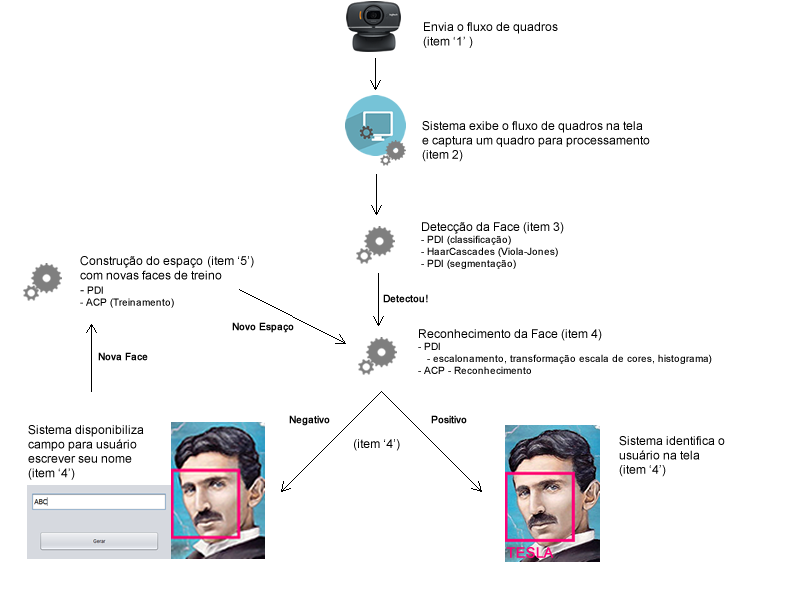
\includegraphics[width=1.12\textwidth]{ilustracao_tcc_sistema}
	\caption{Ilustração do processo do sistema.}
	\fonte{Elaborado pelo autor.}
	\label{fig:ilustracao}
\end{figure}

\begin{enumerate}
	\item \textbf{entrada:} uma câmera do tipo \textit{webcam}, descrita na \autoref{sec: tec-ferramenta}, deve estar filmando uma área com iluminação controlada, produzindo o fluxo de \textit{frames} e disponibilizando em formado digital para o sistema;
	
	\item \textbf{processamento/saída:} o sistema adquire controle do fluxo de \textit{frames} da \textit{webcam}, manipulando-o para que se possa ser exibido na tela do microcomputador e separa um quadro para a detecção, em tempo real, utilizando o algoritmo, descrito na \autoref{subsubsec:violajones}, com os materiais contemplados na \autoref{subsec:bib_opencv};
	
	\item \textbf{processamento:} o sistema processo a detecção da face na imagem, e caso seja detectada uma face, o sistema deverá desenhar um retângulo em volta da face detectada neste fluxo de \textit{frames}, e a partir daí se inicia o processo de reconhecimento;
	
	\item \textbf{processamento/saída:} o processo de reconhecimento é acionado e caso a face não seja reconhecida, o sistema disponibiliza campos para que o usuário entre com uma identificação. Caso haja alguma equivalência, o sistema identifica o usuário escrevendo seu nome logo abaixo do retângulo desenhado pelo processo de detecção;
	
	\item \textbf{entrada/processamento:} se o usuário identifica a face a partir do item acima descrito, o sistema inicia o processo de treinamento da face definido na \autoref{sec:recog_faces}, criando um \textit{eigenspace}, e no momento seguinte à criação deste "espaço", o sistema começa a utiliza-lo para os novos processos de reconhecimento.
\end{enumerate}

\section{Diagrama de Caso de Uso}\label{sec:diagpacs}

O diagrama de Caso de Uso da \autoref{casouso} ilustra a interação entre o usuário (ator) e o sistema. Observa-se que as únicas atividades do usuário é de se posicionar para que a câmera capture as imagens, e preencher o campo disponibilizado para identificação, caso o usuário deseje.

\begin{figure}[h]
	\centering
	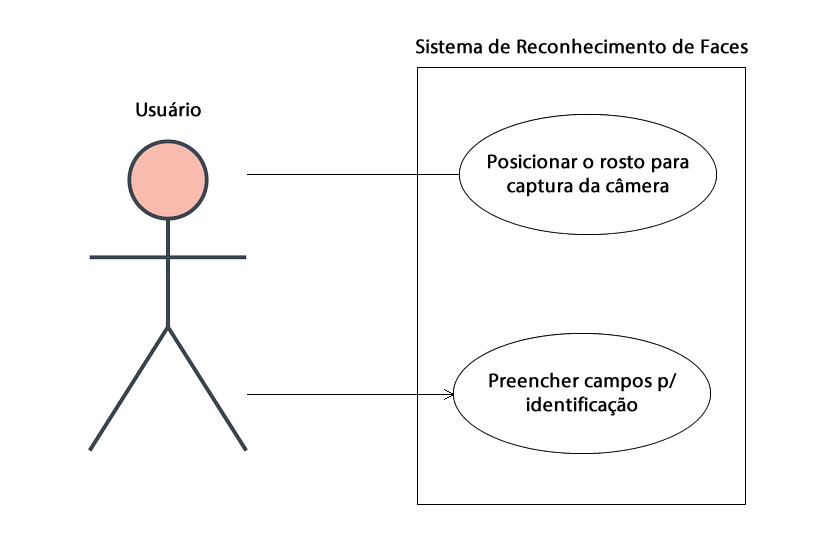
\includegraphics[width=0.9\textwidth]{casouso}
	\caption{Diagrama de Caso de Uso - Interação entre o usuário e o sistema.}
	\fonte{Elaborado pelo autor.}
	\label{casouso}
\end{figure}



\section{Diagrama de Pacotes}\label{sec:diagpacs}
Nesta seção, os pacotes criados para implementação do sistema aqui proposto serão apresentados em forma de diagrama de pacotes UML. A \autoref{fig:SRFV_diagramaPacotes} ilustra tal diagrama:

\begin{figure}[h]
	\centering
	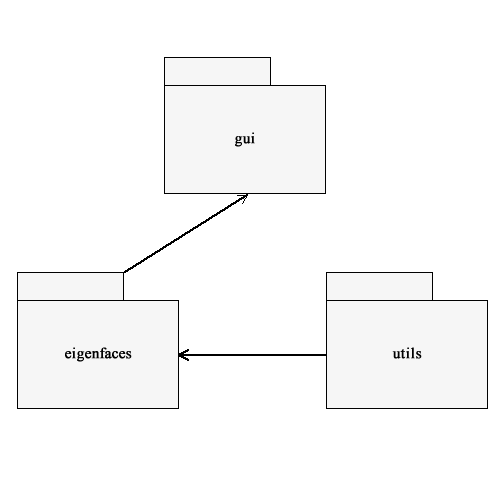
\includegraphics[width=.6\textwidth]{SRFV_diagramaPacotes}
	\caption{Diagrama de pacotes UML do sistema proposto.}
	\fonte{Elaborado pelo autor.}
	\label{fig:SRFV_diagramaPacotes}
\end{figure}

O pacote \textit{"gui"} possui classes responsáveis pela interface com o usuário e regras do sistema como controle de fluxo de quadros e execução de tarefas. O pacote \textit{"eigenfaces"} possui as classes responsáveis pela execução do algoritmo ACP e a geração do espaço multidimensional de \textit{eigenfaces}. Por fim, o pacote de nome \textit{"utils"}, possui classes utilitárias resposáveis por manipular arquivos (carregar, salvar e deletar) e conversões de formatos de imagens. 

Na seção seguinte, cada pacote será descrito com seus respectivos diagramas de classe.

\section{Diagrama de Classes - Pacote \textit{\textbf{gui}}}\label{sec:diagclasses}
As classes do pacote \textbf{\textit{gui}} são representadas pelo diagrama UML na \autoref{figSRFV_diagramaClassse_gui}.

\begin{figure}[h]
	\centering
	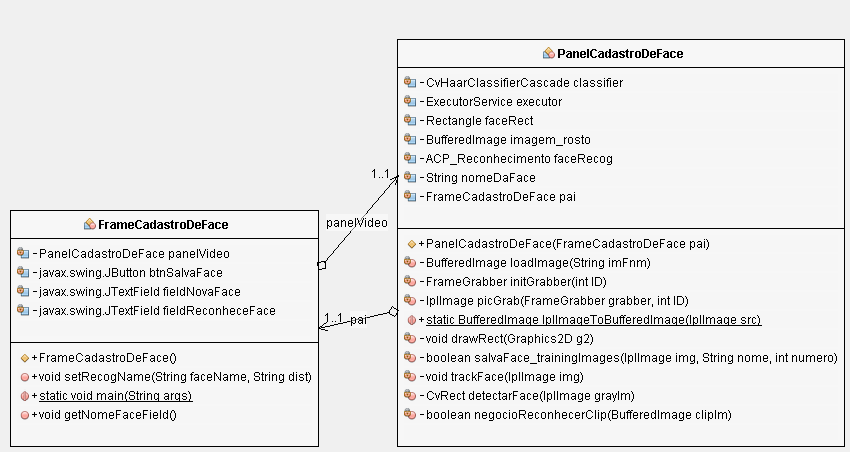
\includegraphics[width=1.1\textwidth]{SRFV_diagramaClassse_gui}
	\caption{Diagrama de classes UML do pacote \textbf{\textit{gui}}.}
	\fonte{Elaborado pelo autor.}
	\label{figSRFV_diagramaClassse_gui}
\end{figure}

A classe \textbf{\textit{FrameCadastroDeFace}} é apenas uma janela com alguns componentes visuais, como um botão, um campo para entrada de informação e a tela para a visualizaçào do fluxo de quadros. A tela para visualização do fluxo é representada pela classe \textbf{\textit{PanelCadastroDeFace}}.

A classe \textbf{\textit{PanelCadastroDeFace}} também é responsávem pelo controle de frames e de execução de tarefas como a de deteção, treinamento e reconhecimento das faces. A seguir suas principais objetos e métodos são detalhados:

\begin{itemize}
	\item Objetos:
	\begin{itemize}
		\item \textbf{CvHaarClassifierCascade classifier}: classificadores pré treinados, assim como descritos na \autoref{subsubsec:violajones}, para o processo de detecção da face;
		
		\item \textbf{ExecutorService executor:} este objeto é uma \textit{thread}, responsável por executar e controlar o processo de aquisiçao de quadros, deteção treinamento e reconecimento;
		
		\item \textbf{Rectangle faceRect:} objeto contendo a posição da face recem detectada em relação ao quadro retirado do vídeo;
		
		\item \textbf{BufferedImage imagem\_rosto:} objeto que salva um a imagem da face, caso detectada;
		
		\item \textbf{String nomeDaFace:} objeto que salva o nome da face detectada, informação esta que é entrada pelo usuário do sistema;
		
		\item \textbf{FrameCadastroDeFace pai:} objeto que referencia o seu parente de nível superior da classe \textbf{\textit{PanelCadastroDeFace}};
		
		\item \textbf{ACP\_Reconhecimento faceRecog:} objeto que instancia a classe responsável por executar o algoritmo de reconhecimento ACP, contido no pacote \textbf{\textit{eigenfaces}};
		
		\item \textbf{ACP\_Treinamento:} esta classe, contida no pacote \textbf{eigenfaces}, não é instanciada como objeto, porém é chamada de forma estática para produzir o espaço multidimensional a partir das imagens de treinamnto salvas em uma pasta especifica;
		
	\end{itemize}
	
	\item Métodos:
	\begin{itemize}
		\item \textbf{BufferedImage loadImage():} método que carrega imagem do sistema de arquivos para memória;
		
		\item \textbf{FrameGrabber initGrabber():} estabelece fluxo de quadros com a câmera;
		
		\item \textbf{IpiImage picGrab():} aquisita um quadro proveniente do fluxo de quadros;
		
		\item \textbf{void drawRect():} desenha um quadrado em volta do rosto aquisitado de acordo com as coordenadas do objeto \textbf{faceRect};
		
		\item \textbf{void salvaface\_traininImages()}: este método salva a face continda no objeto \textbf{imagem\_rosto} para futuro processo de treinamento;
		
		\item \textbf{void trackFace():} método chamado dentro da \textit{thread} ExecutorService executor que contém os processos e os controles de estado de detecção, treinamento e reconhecmento da face;
		
		\item \textbf{boolefan recogFace():} método chamado quando o sistema se encontra no estado de reconhecimento, onde a imagem passa por processamento, redimensionando-a e transformando-a em escala de cinza e passada para o método o objeto \textbf{ACP\_Reconhecimento.processaReconhecimento()} é acionado;
		
		\item \textbf{boolean negocioReconhecerClip():} sub-método do método \textit{recogFace()} definido acima, chamado quando o sistema se encontra no estado de reconhecimento, onde a imagem passa por conversões de tipo,  aciona efetivamente \textbf{ACP\_Reconhecimento.processaReconhecimento()} e determina se o reconhecimento foi um sucesso ou uma falha, detalhado posteriormente na autoref{sec:defsucregoc}, passando os dados de reconhecimento para a interface;
	\end{itemize}
\end{itemize}





\section{Diagrama de Classes - Pacote \textit{\textbf{eigenfaces}}}\label{sec:eigenfacesclass}
As classes do pacote \textbf{\textit{eigenfaces}} são representadas pelo diagrama UML da \autoref{figSRFV_diagramaClassse_eigenfaces} e descritas em seguida. 

\begin{figure}[h]
	\centering
	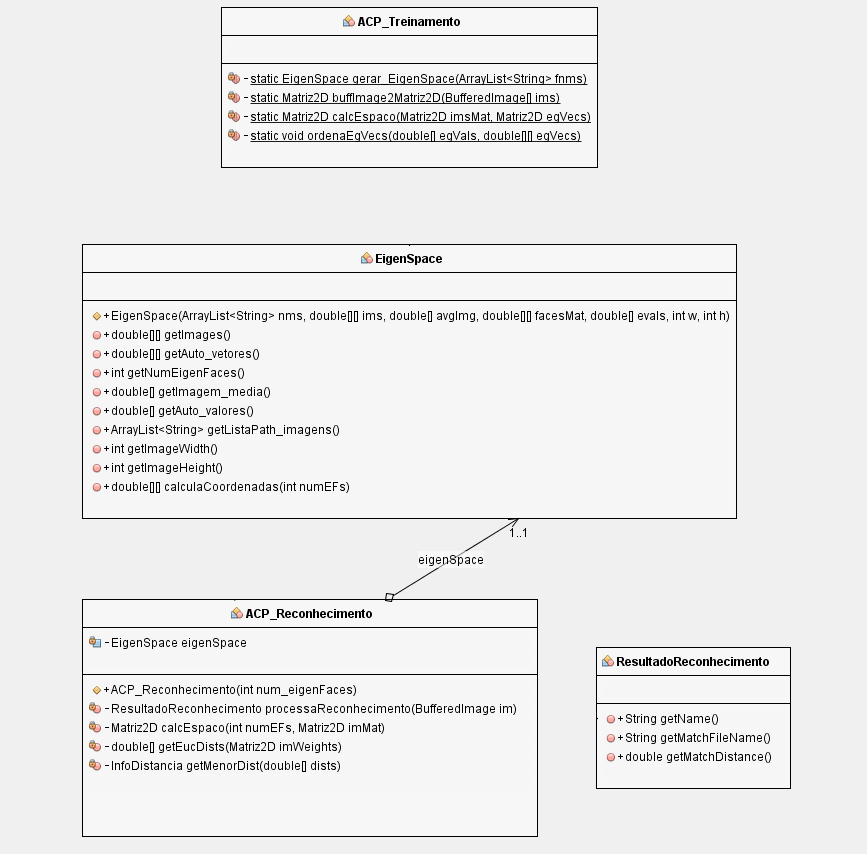
\includegraphics[width=1.1\textwidth]{SRFV_diagramaClassse_eigenfaces}
	\caption{Diagrama de classes UML do pacote \textbf{\textit{eigenfaces}}.}
	\fonte{Elaborado pelo autor.}
	\label{figSRFV_diagramaClassse_eigenfaces}
\end{figure}

%CLASSE EIGENSPACE

A classe \textit{\textbf{EigenSpace}} representa o espaço multidimensional citado e descrito na  \autoref{sec:recog_faces}. Possui métodos de extração de informações contidas neste espaço. Seus objetos são matrizes que representam os autovalores e autovetores contemplados na \autoref{subsec:treinamento}. També possui objetos que relacionam os autovetores gerados com as suas respectivas imagens de treinamento.


\begin{itemize}	
	\item Métodos:
	\begin{itemize}
		\item \textbf{double[][] getImages():} método que retorna as imagens de treinamento em forma de matriz de bytes de duas dimensões. Cada linha representa uma imagem, e o número de colunas representa os pixels de cada imagem;
		
		\item \textbf{double[][] getAutoVetores():} método que retorna os autovetores gerados a partir das imagens de treinamento;
		
		\item \textbf{int getNumEigenFaces():} este método retorna o número de \textit{eigenfaces} presentes no espaço multidimensional \textit{EigenSpace}.
		
		\item \textbf{double[] getImagem\_media():} este método retorna o número de \textit{eigenfaces} presentes no espaço multidimensional \textit{EigenSpace}.
		
		\item \textbf{double[] getAuto\_valores():} retorna os autovalores correspondentes com os autovetores existentes no espaço;
		
		
		\item \textbf{ArrayList<String> getListaPath\_images():} returna uma lista com o caminho completo dos arquivos que representam as imagens de treinamento;
		
		\item \textbf{double[][] calculaCoordenadas(int numEFs):} este método recebe o número de \textit{eigenfaces} a se priorizar para analise, como explica a \autoref{subsec:treinamento}, e retorna as coordenadas (ou pesos) respectivos a cada imagem de treinamento;		
	
	\end{itemize}
\end{itemize}

%CLASSE ACP_TREINAMENTO

A classe \textit{\textbf{ACP\_Treinamento}} contém a implementação responsável pelo processo de treinamento do ACP descrito na \autoref{subsec:treinamento}. Portanto esta classe gera um objeto da classe \textbf{EigenSpace} descrita acima. Seus principais métodos são contemplados abaixo:


\begin{itemize}	
	\item Métodos:
	\begin{itemize}
		\item \textbf{EigenSpace gerar\_EigenSpace():} este método engloba os cálculos do algoritmo ACP, especificamente os passos da fase de treinamento da \autoref{subsec:treinamento}, retornando um objeto da classe \textit{EigenSpace} detalhada anteriormente. 
		
		\item \textbf{Matriz2D calcEspaco():} este método engloba especificamente o passos '5' da fase de treinamento referente ao cálculo do espaço, contempladas na \autoref{subsec:treinamento}.
		
		\item outros métodos para conversão de objetos da classe \textit{Double} para o tipo primitivo \textit{double}, conversão de imagens representadas pela classe \textit{BufferedImage} para \textit{DoubleMatrix2D}, contemplada na \autoref{subsec:bib_colt}, etc.
		
	\end{itemize}
\end{itemize}


%CLASSE ACP_RECONHECIMENTO

A classe \textit{\textbf{ACP\_Reconhecimento}} contém a implementação responsável pelo processo de reconhecimento da ACP descrito na \autoref{subsec:reconhecimento}. Portanto esta classe gera um objeto da classe \textbf{ResultadoReconhecimento} posteriormente nesta seção. Seus principais métodos são contemplados abaixo:


\begin{itemize}	
		\item Objetos:
	\begin{itemize}
		\item EigenSpace eigenSpace: objeto da Classe \textbf{\textit{EigenSpace}}, descrita acima nesta seção, criada pela Classe \textit{ACP\_Treinamento} e utilizada para a fase de reconhecimento.
	\end{itemize}
	
	
	\item Métodos:
	\begin{itemize}
		\item \textbf{void processa\_Reconhecimento():} este método engloba os cálculos do algoritmo ACP, especificamente os passos da fase de reconhecimento da \autoref{subsec:reconhecimento}.
		
		\item \textbf{Matriz2D calcEspaco(int nEF, Matriz2D imMat)}:
		
		\item \textbf{double[] getEucDists(Matriz2D im)}: método que calcula a distância euclidiana de todas as faces treinadas (autovalores) contidos no espaço com a nova face;
		
		\item \textbf{ResultadoReconhecimento getMenorDist(double[] dists)}: método que retorna qual das distâncias calculadas acima é a menor, construindo um objeto da classe \textit{\textbf{ResultadoReconhecimento}};
		
		\item esta classe também contém métodos para conversões de tipos, dentre outros.
		
		
	\end{itemize}
\end{itemize}



%CLASSE ResultadoReconhecimento
A classe \textit{\textbf{ResultadoReconhecimento}} representa o resultado do reconhecimento procesada pela classe ACP\_Reconhecimento contemplada anteriormente. Seus principais métodos são detalhados abaixo:


\begin{itemize}	
	\item Métodos:
	\begin{itemize}
		\item \textbf{String getName():} método que retorna a identificação da face previsamente informada pelo usuário, correspondente com o resultado;		
		\item \textbf{String getMatchFileName():} método que retorna o caminho do arquivo que corresponde ao resultante.
		\item \textbf{BufferedImage getMatchDist():} método que retorna distância corresponde com o resultado;
	\end{itemize}
\end{itemize}





\section{Diagrama de Classes - Pacote \textit{\textbf{utils}}}\label{sec:ituls}
As classes do pacote \textbf{\textit{utils}} são representadas pelo diagrama UML da \autoref{figSRFV_diagramaClassse_utils}. 

\begin{figure}[h]
	\centering
	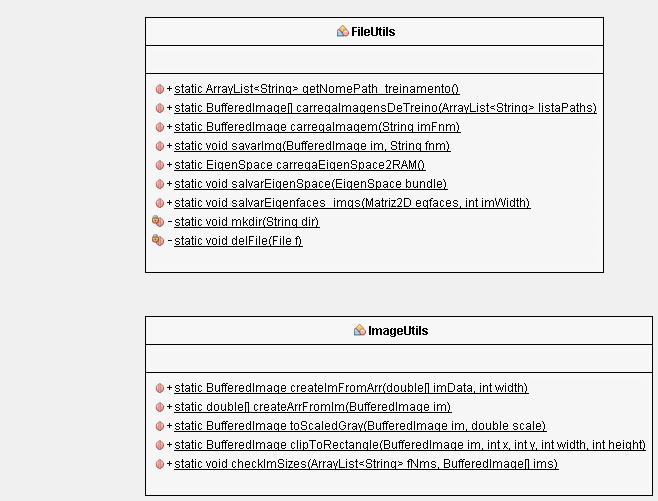
\includegraphics[width=1.1\textwidth]{SRFV_diagramaClassse_utils}
	\caption{Diagrama de classes UML do pacote \textbf{\textit{utils}}.}
	\fonte{Elaborado pelo autor.}
	\label{figSRFV_diagramaClassse_utils}
\end{figure}

%CLASSE FileUtils
A classe \textit{\textbf{FileUtils}} contém métodos que carregam arquivos do disco rígido para a memória, conversão entre classes de imagem, e também que salvam as imagens contidas na memória para o disco rígido, dentro outros como remoção de arquivos e manipulação de pastas.


%CLASSE ImageUtils
A classe \textit{\textbf{ImageUtils}} contém métodos que responsáveis por algumas rotinas de processamento de imagens. Seus principais métodos são descritos abaixo:


\begin{itemize}	
	\item Métodos:
	\begin{itemize}
		\item \textbf{String clipToRectangle(BufferedImage, int, int, int, int):} este método recebe uma imagem e quatro pontos, e segmenta a imagem de acordo com estes parâmetros;
		
		\item \textbf{BufferedImage escalaImagemCinza(BufferedImage, double ):} recebe uma imagem, a escalona para proporcionalmente de acordo com um parâmetro constante de escala e retorna outra imagem representada pela classe BufferedImage, já transformada para escala de cores cinza;
		
		\item \textbf{BufferedImage escalaImagemCinza(IpiImage)}: apresenta a mesma finalizade do método acima porém recebendo um objeto da classe IpiImage da biblioteca OpenCV descrita na \autoref{subsec:bib_opencv}, retornando outra imagem representada pela classe BufferedImage, já transformada para escala de cores cinza;
		
		\item esta classe também possui métodos de conversão de vetores para o tipo \textit{BufferedImage }e vice-versa.
	\end{itemize}
\end{itemize}


%CLASSE Auto vetod decomposicao
A classe \textit{\textbf{AutoVetor\_decomp}} herda as propriedades da classe \textit{EigenvalueDecomposition} da biblioteca \textit{COLT} contemplada na \autoref{subsec:bib_colt}, responsável por decompor uma matriz de covariância em autovalores e autovetores, como detalha a \autoref{subsec:treinamento}.


%CLASSE equ histogra
A classe \textit{\textbf{EqualizarHistograma}} é responsável por processar a equalização de histogramas em todas as imagens de treinamento, as quais são salvas pela classe \textit{FileUtils} em uma pasta definida no disco rígido.


%CLASSE equ histogra
Por fim, a classe \textit{\textbf{Matriz2D}} herda a propriedades da classe \textit{\textbf{DoubleMatriz2D }} da biblioteca \textit{COLT}, responsável por representar matrizes com funções para calculá-las. Contém métodos de conversões de tipos e cálculo de matrizes. Seus principais métodos são detalhados abaixo, os quais herdam as funcionalidades contempladas na \autoref{subsec:bib_colt}:
\begin{itemize}	
	\item Métodos:
	\begin{itemize}
		\item \textbf{void subtract(Matriz2D):} este método recebe uma matriz a ser subtraída e realizar o cálculo;
		
		\item \textbf{String max(double[]):} recebe um vetor e retorna seu maior valor;
		
		\item \textbf{void normalise():} normaliza a objeto matriz representada por esta classe;
		
		\item \textbf{void transpose():} realiza o processo de transposição da matriz representada por esta classe;
		
		\item \textbf{double[] calcMedia\_cols():} calcula a média das colunas da matriz representada por esta classe, retornando um vetor com os estes valores médios.
		
		\item \textbf{\textit{void subtrairMedia()}:} este método faz a chamada do método acima descrito 		 \textit{calcMedia\_cols} e a subtrai com a matriz representada por esta classe, tendo como resultado um vetor médio subtraído, ou face média subtraída, como descreve a \autoref{subsec:treinamento}.

	\end{itemize}
\end{itemize}




Para melhor visualização e entendimento da relação entre estas classes e seus métodos, apresenta-se na \autoref{diagsequencia} o diagrama de sequência das classes \textit{ACP\_Treinamento}, \textit{Matriz2D}, \textit{FileUtils} e \textit{EqualizarHistograma}. Também apresenta-se o diagrama de sequência das classes \textit{Matriz2D}, \textit{AutoVetor\_decomp}, \textit{DenseDoubleMatriz} e  \textit{EigenValueDecomp}, sendo estas duas últimas, classes pertencentes à biblioteca Colt, contemplada na \autoref{subsec:bib_colt}. Os detalhes das operações executadas por estes métodos serão contemplados na \autoref{sec:codigo}.


\begin{figure}[h]
	\centering
	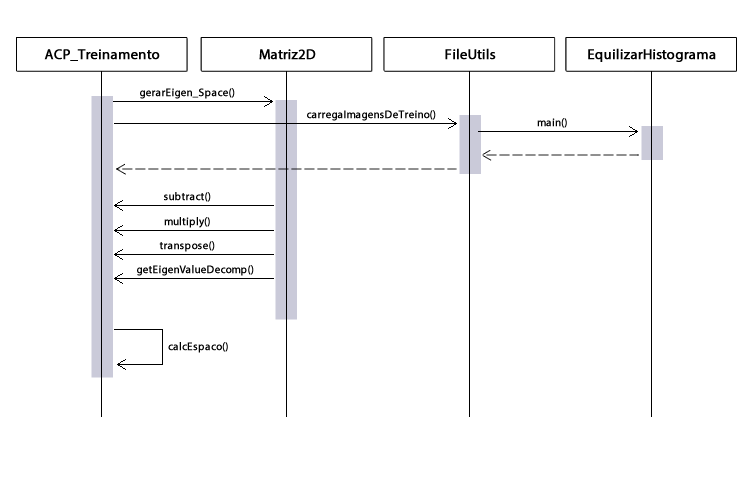
\includegraphics[width=0.9\textwidth]{diagsequencia}
	\caption{Diagrama de sequência UML  das classes \textit{ACP\_Treinamento}, \textit{Matriz2D}, \textit{FileUtils} e \textit{EqualizarHistograma}.}
	\fonte{Elaborado pelo autor.}
	\label{diagsequencia}
\end{figure}


\begin{figure}[h]
	\centering
	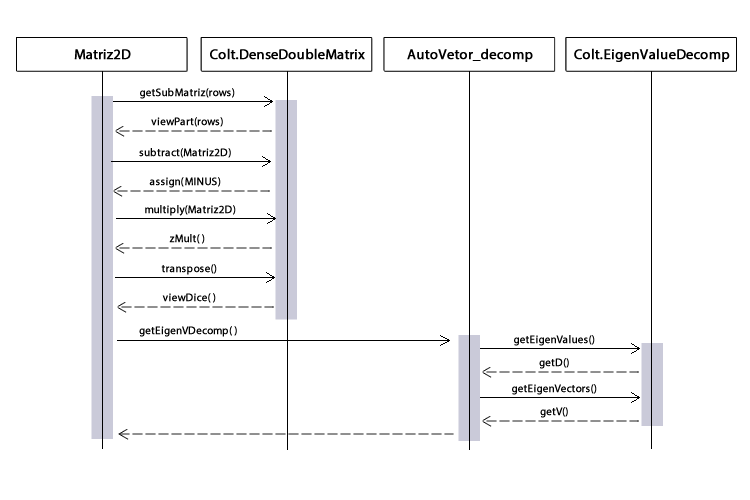
\includegraphics[width=0.9\textwidth]{diagsequenciaMatrixOP}
	\caption{Diagrama de sequência UML  das classes \textit{Matriz2D}, \textit{AutoVetor\_decomp}, \textit{DenseDoubleMatriz} e  \textit{EigenValueDecomp}.}
	\fonte{Elaborado pelo autor.}
	\label{diagsequenciaMatrixOP}
\end{figure}



%CODIGO!!!
\section{Implementação do Código}\label{sec:codigo}

Nesta seção será abordado a implementação do código, definindo quais foram as variáveis (ou constantes em termos de programação) pré-estabelecidas e constroladas para o obter diversos efeitos ou resultados, como define o método experimentao descrito na \autoref{metex}.

Também serão contemplados os \textit{snippets} (ou blocos de código) referentes às principais partes implementadas do sistema e descritas neste trabalho: o fluxo do processo do sistema como ilustra na \autoref{fig:ilustracao} da \autoref{sec:analiserec}, a fase de treinamento e a de reconhecimendo do algoritmo EigenFaces (ACP), descritos na \autoref{subsec:acp}.

\subsection{Constantes Controladas}\label{sec:consts}

De acordo com o método experimental, utilizou-se três constantes controladas como variáveis do experimento, para que sejam manipulados e seus efeitos obervados. Existem outras constantes no sitema para constrole de quadros analisados ou do tamanho padrão da imagem que tem efeito no desempenho ou em outros aspectos do sistema, porém os três principais listados abaixo influem na taxa de sucesso/falha do reconhecimento, os quais serão contemplados no \autoref{ch:resultados}, referente aos testes e resultados.

\begin{itemize}	
		\item \textbf{NUM\_FACES\_TREINO:} esta constante é resposável por controlar o número de faces a ser usado no treinamento, acionado quando o usuário informa sua identificação. Apresenta-se sua lógica no código na \autoref{sec:mainthread};
		
		\item \textbf{NUM\_EF\_recog:} esta constante é responsável por definir quantos autovetores serão utilizados para o reconhecimento, pois seu descarte é possível devido a ordenação por autovalores, como contempla a \autoref{subsec:treinamento}, passo quatro, e a \autoref{sec:implrecog}. Sua lógica é apresentada na \autoref{sec:implrecog};
		
		\item \textbf{MIN\_DIST:} esta constante define se a distância encontrada na fase de reconhecimento pode ser considerada um resultado de sucesso ou falha. Sua lógica apresentada na \autoref{sec:defsucregoc}.
\end{itemize}


\subsection{Processo Principal do Sistema}\label{sec:mainthread}

O bloco do \autoref{snippet-mainthread} corresponde a \textit{Thread} (classe para processamento paralelo) que controla o fluxo do sistema que se refere aos processos de detecção, treinamento e reconhecimento da imagem capturada do fluxo de quadros, disponibilizadas pela \textit{webcam}.

%\begin{figure}[h]
%	\centering
%	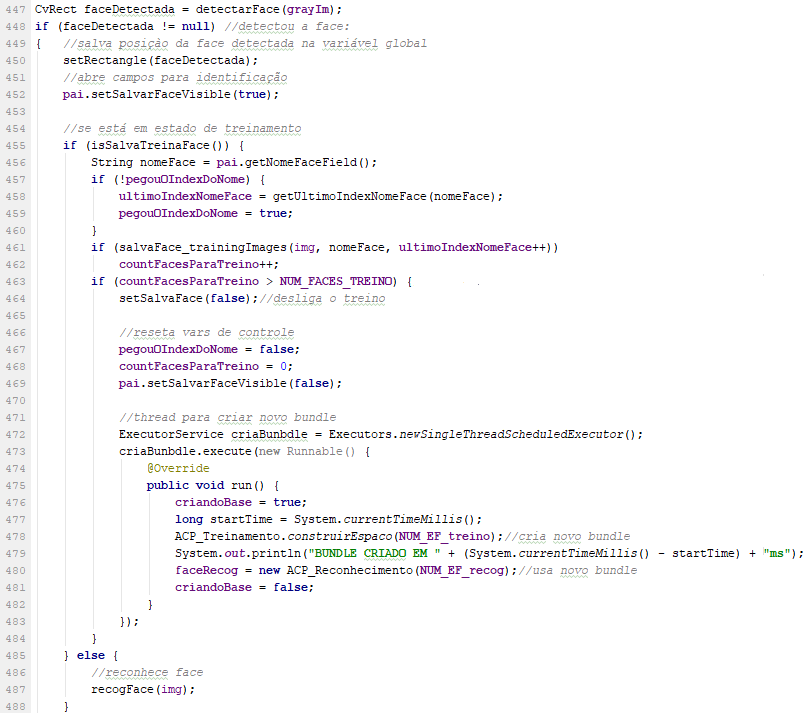
\includegraphics[width=1\textwidth]{snippet-mainthread}
%	\caption{Bloco de código do método \textit{trackFace()} da classe \textit{PanelCadastroDeFace}}
%	\fonte{Elaborado pelo autor.}
%	\label{snippet-mainthread}
%\end{figure}



\codigoJava
\lstinputlisting[firstnumber=447, language=Java, label=snippet-mainthread, caption=Bloco de código do método \textit{trackFace()} da classe \textit{PanelCadastroDeFace}]{src/snippet-mainthread.java}


Este bloco está contido do método \textit{trackFace()} da classe \textit{PanelCadastroDeFace}, descritas na \autoref{sec:diagclasses}, que é chamado a cada captura de quadros, atribuindo como parâmetro a image já redimensionada e transformada para cores da escala cinza, como mostra o  \autoref{snippet-mainthread}.

A linha de número \textit{447}, o método \textit{detectarFace(grayIm)} recebe uma imagem já redimensionada e transformada em escala da cinza pelo método \textit{escalaImagemCinza()}, descrito na \autoref{sec:ituls}, e processa a detecção da face utilizando o algoritmo de Viola-Jones (descritos na \autoref{subsubsec:violajones}). Se a face não for detectada, nada acontece. Caso a face seja detectada na imagem, as coordenadas desta são salvas em uma variável global e os campos de identificação contidos na classe \textit{FrameCadastroFace} para identificação do usuário são ativados  (linha \textit{450} e \textit{452}, respectivamente). 

Caso o usuário se identifique atravéz dos campos de entrada, o sistema se encontrará em "estado de treinamento", controlado pelo método \textit{isSalvaTreinaFace()} da linha 455. Neste bloco salva-se a imagem da face para treino quantas vezes for definida pela constante \textit{NUM\_FACES\_TREINO}, definidas na \autoref{sec:consts}. Quando atingir este valor, o "estado de treinamento"\ do sistema, bem como os campos de entrada são desativados e começa a rotina de construção do espaço (\textit{eingenspace}), executada pelo método \textit{ACP\_Treinamento.construirEspaco()}, que será detalhado em seguida nesta seção.

Se o sistema não se encontra em "estado de treinamento", controlado pelo método \textit{isSalvaTreinaFace()} da linha \textit{445}, o método \textit{recogFace()} (linha \textit{487}) é executado, o qual será detalhado na \autoref{sec:implrecog}.


\subsection{Fase de Treinamento}\label{sec:impltrein}
%\begin{figure}[h]
%	\centering
%	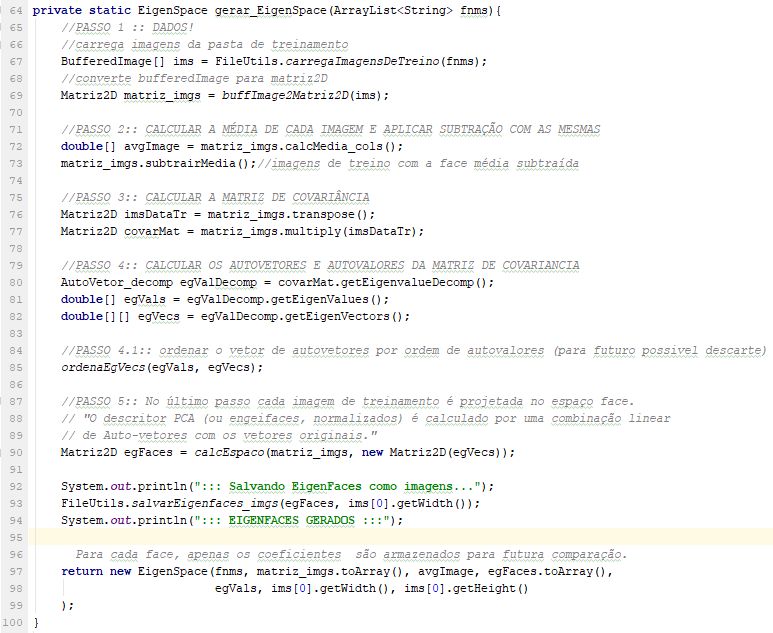
\includegraphics[width=1\textwidth]{snippet-treiamento}
%	\caption{Bloco de código do método \textit{gerar\_EigenSpace()} da classe \textit{ACP\_Treinamento}}
%	\fonte{Elaborado pelo autor.}
%	\label{snippet-treiamento}
%\end{figure}


O método \textit{gerar\_EigenSpace()} do \autoref{snippet-treiamento} é chamado pelo método \textit{ACP\_Treinamento.construirEspaco()}, contemplado no bloco de código anterior, que por sua vez resgata todas as imagens de treino, salvar em disco rígido e retorna os caminhos destes arquivos.

\codigoJava
\lstinputlisting[firstnumber=64, language=Java, label=snippet-treiamento, caption=Bloco de código do método \textit{gerar\_EigenSpace()} da classe \textit{ACP\_Treinamento}]{src/snippet-treiamento.java}


Este bloco é o responsável por executar a fase de treinamento do algoritimo ACP (ou \textit{EigenFaces}), contemplada na seção \autoref{subsec:treinamento}, e seus cinco passos:

No primeiro passo, carrega-se as imagens do disco rígido para a memória e as converte para as classes que as representam em matrizes (linha \textit{67} e \textit{69}). 

Para o segundo passo, o cálculo da face média é executado e subtrai-se esta com a matriz criada no primeiro passo, como está nas linhas \textit{72} e \textit{73} do  \autoref{snippet-treiamento}.

No terceiro passo, o vetor de covariância é calculado multiplicando a matriz gerada no passo anterior com sua equivalente transposta, como contempla a \autoref{subsec:treinamento} (linhas \textit{76} e \textit{77}).

No quarto passo deve-se decompor a matriz de covariância em autovalores (\textit{eigenvalues}) e autovetores (\textit{eigenvectors}). Isto é feito atravéz dos métodos \textit{getEigenValues()} e \textit{getEigenVectors()} (linhas \textit{81} e \textit{82}, respectivamente) da classe \textit{AutoValor\_decomp}, descritas na \autoref{sec:ituls}, e posteriormenter ordenados por ordem de autovalores (linha \textit{85}).

%\begin{figure}[h]
%	\centering
%	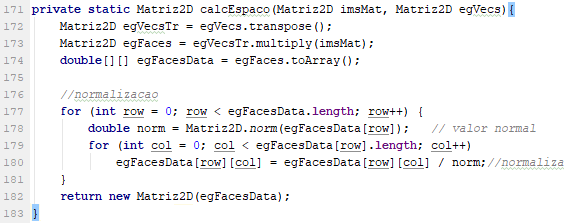
\includegraphics[width=0.8\textwidth]{snippet-treiamento-calcesp}
%	\caption{Bloco de código do método \textit{calcEspaco()} da classe \textit{ACP\_Treinamento}, responsável por executar o quinto passo da fase de treinamento.}
%	\fonte{Elaborado pelo autor.}
%	\label{snippet-treiamento-calcesp}
%\end{figure}


Para o quinto e último passo desta fase de treinamento, o cálculo do espaço (\textit{eigenspace}) é executado atravéz do método \textit{calcEspaco()}, descritos no bloco do \autoref{snippet-treiamento-calcesp}. 


\codigoJava
\lstinputlisting[firstnumber=171, language=Java, label=snippet-treiamento-calcesp, caption=Bloco de código do método \textit{calcEspaco()} da classe \textit{ACP\_Treinamento} - responsável por executar o quinto passo da fase de treinamento.]{src/snippet-treiamento-calcesp.java}


\subsection{Fase de Reconhecimento}\label{sec:implrecog}

O método \textit{processaReconhecimento()} contemplado no bloco do \autoref{snippet-reconh}, é responsável por executar os três passos da fase de reconhecimento do algoritmo \textit{Eigenfaces} (ACP), descritos na \autoref{subsec:reconhecimento}.

%\begin{figure}[h]
%	\centering
%	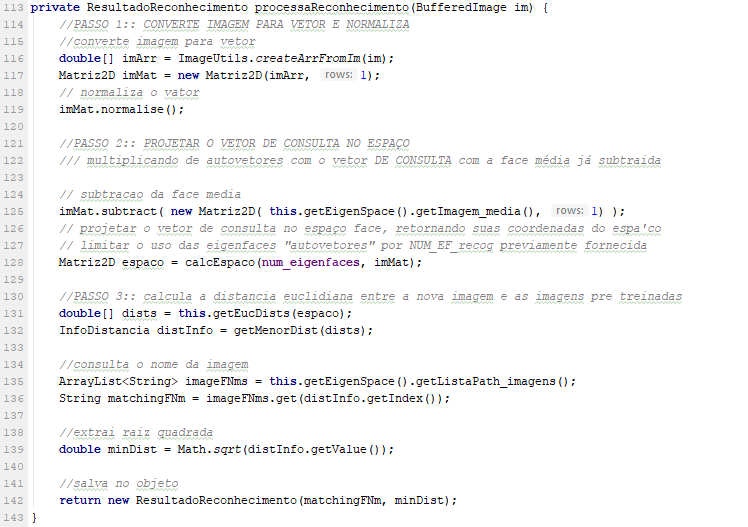
\includegraphics[width=1.05\textwidth]{snippet-reconh}
%	\caption{Bloco de código do método \textit{processaReconhecimento()} da classe \textit{ACP\_Reconhecimento}}
%	\fonte{Elaborado pelo autor.}
%	\label{snippet-reconh}
%\end{figure}


\codigoJava
\lstinputlisting[firstnumber=113, language=Java, label=snippet-reconh, caption=Bloco de código do método \textit{processaReconhecimento()} da classe
\textit{ACP\_Reconhecimento}]{src/snippet-reconh.java}


O método \textit{regocFace()} da classe \textit{PanelCadastroDeFace}, como descrito na da \autoref{sec:diagclasses}, invoca este método \textit{processaReconhecimento()} para fazer o reconhecimento, passando imagem da classe \textit{BufferedImage} já processada, que representa a nova face a ser reconhecida. 

Para o primeiro passo da fase de reconhecimento, prepara-se os dados para o cálculo fazendo conversão entre classes (linha \textit{116} e \textit{117}), e normaliza a matriz que representa a nova imagem com a média dos próprios valores (linha \textit{119}).

No segundo passo projeta-se o novo vetor de consulta ao espaço previamente criado na fase de treinamento. Para isto, é necessário extrair a face média do espaço, previamente salva no objeto da classe \textit{eigenspace}, e subtraí-la do vetor de consulta (linha \textit{125} do \autoref{snippet-reconh}) para que seja atendida a equação de definição do espaço com o novo vetor de consulta, detallhada  na \autoref{subsec:reconhecimento}. 

O método \textit{calcEspaco()} (linha \textit{128} do \autoref{snippet-reconh}), semelhante ao método \textit{calcEspaco()} da classe \textit{ACP\_Treiamento}, é responsável pelo cálculo do novo espaço com o novo vetor de consulta, detalhado e ilustrado no bloco de código do \autoref{snippet-reconh-calcesp}. Nele recupara-se os autovalores contidos no espaço previamente criado pela fase de treinamento (linha \textit{150} - \autoref{snippet-reconh-calcesp} ) e se extrai a submatriz determinada de autovalores pela constante \textit{NUM\_EF\_recog}, especificada na \autoref{sec:consts} (linha \textit{151} - \autoref{snippet-reconh-calcesp}), seguidas das operações de transposição e multiplicação (linhas \textit{152} e \textit{154} do \autoref{snippet-reconh-calcesp}), para que se atenda a equação de criação do espaço (\textit{eigenspace}) com o novo vetor de consulta (\autoref{subsec:reconhecimento}).

%\begin{figure}[h]
%	\centering
%	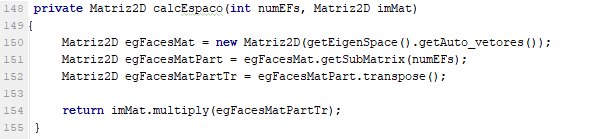
\includegraphics[width=0.85\textwidth]{snippet-reconh-calcesp}
%	\caption{Bloco de código do método \textit{calcEspaco()} da classe \textit{ACP\_Treinamento}}
%	\fonte{Elaborado pelo autor.}
%	\label{snippet-reconh-calcesp}
%\end{figure}

\codigoJava
\lstinputlisting[firstnumber=148, language=Java, label=snippet-reconh-calcesp, caption=Bloco de código do método \textit{calcEspaco()} da classe \textit{ACP\_Treinamento}]{src/snippet-reconh-calcesp.java}


Para o terceiro e último passo da implementação desta fase de reconhecimento, a Distância Euclidiana entre as coordanadas de cada autovetor (\textit{eigenface}) geradas na faze de treinamento e as coordenadas dos mesmos no novo espaço gerados nesta faze são calculados (linha \textit{131} do \autoref{snippet-reconh}), subtraíndo-as e elevando-as ao quadrado. A menor delas é elegida (linha \textit{132} do \autoref{snippet-reconh}) e é calculada sua raiz quadrada para completar a equação da Distância Euclidiana, contemplada na \autoref{subsec:reconhecimento}, criando um objeto da classe \textit{ResultadoReconhecimento}, detalhado na \autoref{sec:eigenfacesclass}, que salva o resultado da melhor distância obtida e a identificação da imagem de treinamento correspondente (a face).


\subsection{Definição de Sucesso do Reconhecimento}\label{sec:defsucregoc}

Como visto na definição do algoritmo \textit{EigenFaces}, disposta na \autoref{subsec:acp}, este apenas apresenta como resultado a menor distância entre os autovetores e o novo vetor de consulta, sendo responsabilidade de outro processo a análise deste resultado para definir se efetivamente este valor corresponte a uma reconhecimento de sucesso ou uma falha.

A constante \textit{MIN\_DIST}, definida na \autoref{sec:consts}, é a responsável pelo resultado final de sucesso ou falha, a qual é controlada e nos testes da \autoref{ch:resultados} posterior. Como mostra o bloco de código do \autoref{snippet-reconh-resultadofim}, a checagem desta constante contra a distância encontrada na fase de reconhecimento pode ser vista na linha \textit{614}.



\codigoJava
\lstinputlisting[firstnumber=607, language=Java, label=snippet-reconh-resultadofim, caption=Bloco de código do método \textit{negocioReconhecerClip()} da classe \textit{PanelCadastroDeFace}]{src/snippet-reconh-resultadofim.java}

%\begin{figure}[h]
%	\centering
%	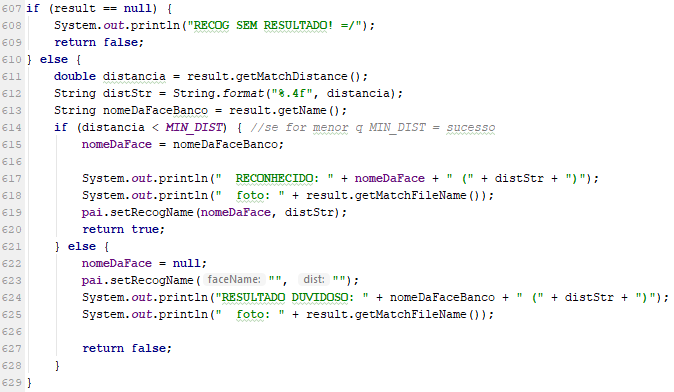
\includegraphics[width=1\textwidth]{snippet-reconh-resultadofim}
%	\caption{Bloco de código do método \textit{negocioReconhecerClip()} da classe \textit{PanelCadastroDeFace}}
%	\fonte{Elaborado pelo autor.}
%	\label{snippet-reconh-resultadofim}
%\end{figure}

Caso a menor ditância calculada seja menor do que a constante \textit{MIN\_DIST}, o resultado é considerado sucesso e os dados correspondentes a este são passados como parâmetro para a interface (linha \textit{619}) para que seja exibido. Tando em caso de sucesso ou de erro, um registro do resultado juntamente com o caminho da imagem correspondente e a distância resultante é realizado (linhas \textit{617}, \textit{618}, \textit{624} e \textit{625}) para futura análise dos resultados, que são apresentados no  \autoref{ch:resultados}.


\subsection{Interface do Sistema}\label{sec:interface}


A \autoref{screenshot-gui} ilustra a interface produzida pela implementação das classes do pacote "gui", e a \autoref{screenshot-sys} representa o sistema em funcionamento, mostrando o fluxo de quadros da câmera na janela do sistema e detectando uma face.

\begin{figure}[h]
	\centering
	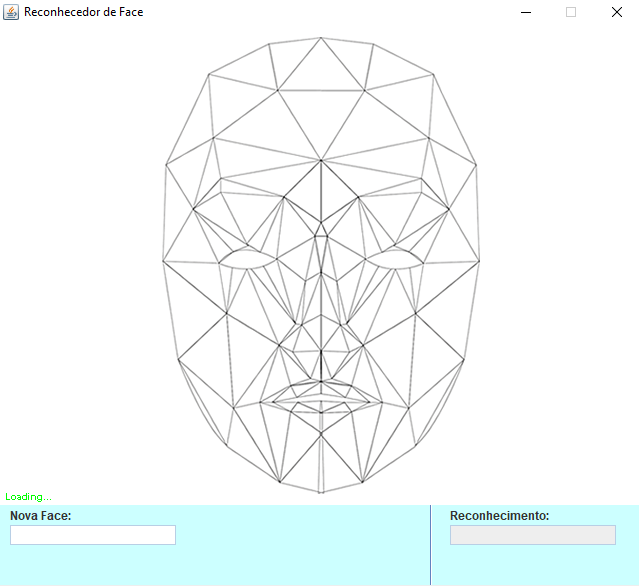
\includegraphics[width=1\textwidth]{screenshot-gui}
	\caption{Imagem da interface do sistema.}
	\fonte{Elaborado pelo autor.}
	\label{screenshot-gui}
\end{figure}


\begin{figure}[h]
	\centering
	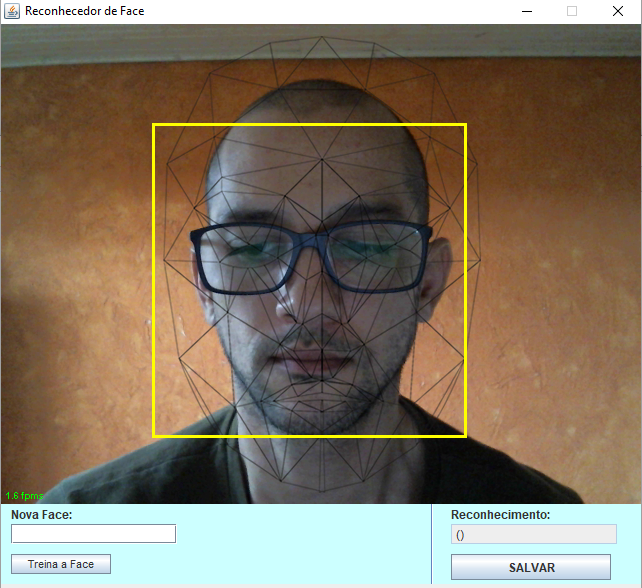
\includegraphics[width=1\textwidth]{screenshot-sys}
	\caption{Imagem do Sistema em Funcionamento.}
	\fonte{Elaborado pelo autor.}
	\label{screenshot-sys}
\end{figure}



Neste capítulo foi apresentado a implementação do código, focando no fluxo de processo do sistema ilustrado e a implementação do algoritmo \textit{EigenFaces}, detalhando suas fases de treinamento e reconhecimento, e a definição do resultado como sucesso ou falha.

No próximo capítulo será apresentado a maneria de como foram controladas as constantes (definidas na \autoref{sec:consts}) nas sessões de testes e seus efeitos como resultados deste experimento.



%\codigoPython
%\lstinputlisting[language=Python, label=coleta-script, caption=\textit{Script} coletar-hashtags.py]{src/coletar-hashtags.py}
